\documentclass[11pt]{article}
\usepackage[utf8]{inputenc}
\usepackage{amsmath, amssymb}
\usepackage{graphicx}
\usepackage{natbib}
\usepackage{geometry}
\usepackage{setspace}
\geometry{margin=1in}
\usepackage{hyperref}
\usepackage{titlesec}
\usepackage{booktabs}  % for \toprule, \midrule, \bottomrule
\usepackage{caption}   % for caption customization if needed
\usepackage{float}
\usepackage{threeparttable}
\usepackage[english]{babel}


\title{UEFA vs FIFA Tie Break: Which Creates More Suspense?}
\author{Alessandro Di Mattia and Alex Krumer}

\date{}   % suppress date

\begin{document}

\maketitle

\begin{abstract}
This study provides both theoretical and empirical support for the definition of suspense in sport, with a particular focus on football. By comparing the tie-breaking rules adopted by UEFA in the European Championship and FIFA in the World Cup, we construct an aggregate measure of suspense at the group level. Our findings show that these rules generate significantly different levels of suspense during the group stage. In particular, the goal-difference criterion used in the FIFA World Cup produces higher group-level suspense, a result that is especially pronounced when applied to the European Championship.

We then examine how suspense evolves over the 90 minutes of play. In the World Cup, groups characterized by high levels of suspense drastically differs from groups with low suspense. Moreover, FIFA's goal-difference rule yields a more stable distribution of goals over time. Finally, we embed our aggregate measure within existing match-level metrics of suspense, surprise, and shock, demonstrating that UEFA’s head-to-head criterion has a stronger impact on match-level fluctuations than FIFA’s, as goals in direct clashes disproportionately influence qualification criteria.
\end{abstract}

% \tableofcontents

\newpage

\section{Introduction}

In the modern era of sports, and football in particular, retaining audience attention has become both more difficult and more crucial than ever before. Spectators today are exposed to a multitude of entertainment alternatives, making the task of sustaining engagement a key factor for the success and profitability of sport organizations. Beyond loyalty to a specific team, fans gain significant enjoyment from \emph{non-instrumental information}—such as the suspense and uncertainty inherent in a match—which fulfills fundamental psychological needs \citep{ely2015suspense, zillmann2013psychology}. This value often drives consumer interest independently of the game’s final result, being rooted instead in the developments that lead to that outcome. \citep{vorderer2004enjoyment}

The economic importance of fan engagement is underscored by the astonishing viewership and revenue generated by major tournaments. For instance, the 2022 FIFA World Cup in Qatar attracted approximately 2.87 billion viewers who watched at least one minute of coverage, while over 5 billion people engaged across broadcast, digital, and social media platforms, 
including 2.9 billion via linear TV and 2.7 billion through digital streaming\citep{fifa2022engagement, fifa2022audience}. Broadcasting and commercial rights from this World Cup cycle generated over USD 6.3 billion for FIFA, representing 83\% of the organization's revenue \citep{fifa2022finance}. 

Similarly, the UEFA European Championship continues to attract massive audiences, with Euro 2024 welcoming a cumulative stadium attendance of 2.67 million across its 51 matches and 5.7 billions of viewers worldwide through television \citep{uefa2024numbers,uefa2024remember}. These figures confirm that maintaining audience attention translates directly into financial success.

Given these stakes, the challenge for sports institutions is not only to increase the number of matches, but to design competitions that maximize suspense and engagement. Low-stakes games may decrease overall interest, while mechanisms that preserve uncertainty—such as tie-breaking rules can extend fan attention across the tournament. Understanding how tie-breaking procedures influence suspense is therefore not only a matter of sporting fairness, but also of monetary relevance, as it directly affects consumer demand, broadcaster revenues, and sponsor value.

In this paper, we investigate how alternative tie-breaking rules influence the level of suspense in international football tournaments. In particular, we compare the two main approaches adopted by governing bodies: FIFA’s adoption of overall goal difference and goals scored, and UEFA’s use of head-to-head results. Building on the established notion of match-level suspense introduced by \citet{bizzozero2016importance}, we extend the analysis to the group stage by developing a measure of suspense at the group level. To enrich this framework, we incorporate additional metrics of surprise and shock, highlighting how their dynamics differ under the two tie-breaking rules. In doing so, we demonstrate that suspense is not solely determined by match dynamics but is also shaped by group-level factors that influence teams’ incentives to win, thereby directly affecting the suspense of the game itself.

\vspace{0.5em}

The structure of the paper is as follows. Section ~\ref{sec:literature} reviews the relevant literature. Section ~\ref{sec:data} presents the data, while Section ~\ref{sec:estimation} outlines the empirical strategy and methodological framework. Section ~\ref{sec:results} reports the results, and Section ~\ref{sec: conclusion} concludes with final remarks.

\section{Literature Review}
\label{sec:literature}

Our paper lies at the intersection of tournament design and the drivers of sport consumption. Recent contributions in sports economics have highlighted critical flaws in the rules and formats of international football competitions, showing how these deficiencies affect both the fairness of outcomes and the demand for the game. For instance, \citet{csato2025increasing} propose a novel framework to evaluate the cost of stake-less  games in which the result no longer influences qualification -- for the newly approved 2026 FIFA World Cup format. Similarly,\citet{lapre2023evolution, lapre2022quantifying} demonstrate how FIFA’s seeding system has consistently failed to reduce competitive imbalance, thereby significantly lowering some teams’ chances of advancing in the competition. As concerns UEFA regulations, \citet{csato2020neither} show how flaws in the qualification rules can create scenarios where teams are incentivized not to win, revealing incentive-compatibility issues in current tournament designs.

To address such structural weaknesses, researchers have advanced a range of solutions, from probabilistic models that improve the predictive accuracy of ranking algorithms \citep{szczecinski2022fifa}, to deterministic optimal scheduling that reduces collusion and stake-less games \citep{chater2021fixing}. Other studies focus on redesigning tournament formats and rules to eliminate misaligned incentives: this includes alternative qualification systems \citep{guajardo2024tournament}, dynamic three-team formats \citep{troyano2023new}, and double-elimination structures \citep{renno2023double}.

\vspace{0.5em}

A related concern arises with the choice of tie-breaking rules, which directly shapes the fairness and stakes of group-stage matches. For example, \citet{berker2014tie} shows that under certain rules, a team’s ranking can depend on the outcome of a match in which it does not participate. Similarly, \citet{csato2023avoid} demonstrates that the likelihood of uncompetitive matches -- where teams lack incentives to exert full effort -- depends strongly on the tie-breaking criteria adopted. These findings highlight that poorly designed tie-breakers not only influence sporting outcomes but also affect the integrity and attractiveness of competitions.

The consequences of these design flaws are not limited to sporting fairness but extend to the economics of sport consumption. Formats and rules that generate collusion opportunities or reduce competitiveness undermine fan interest, diminishing both the entertainment value and commercial revenues of tournaments. Understanding the drivers of demand for both live attendance and broadcast audiences is therefore essential. Several studies identify in-game dynamics as key factors: \citet{buraimo2020unscripted} show that suspense, surprise, and shock capturing the tension and emotional intensity of matches contribute to higher demand, particularly at specific moments of play. Likewise, \citet{alavy2010edge} argue that the progression of the game, rather than its final outcome alone, is crucial, with greater uncertainty about results increasing spectator engagement. Similarly, \citet{bizzozero2016importance} find a strong link between suspense and surprise on the one hand, and the demand for entertainment on the other. Finally, \citet{buraimo2022armchair} extend this perspective to television audiences, showing that demand cannot be explained solely by uncertainty of outcome but also depends on players' quality and the significance of the match (e.g., title races, European qualification, or relegation battles).

Taken together, this domain of research shows that flawed formats and rules do not merely raise ethical and fairness concerns but also undermine the economic value of competitions by reducing engagement and the attractiveness of matches. Our contribution builds on this insight by shifting the perspective to that of the spectator and examining how institutional features -- in particular, tie-breaking rules -- shape the stakes of a match and, ultimately, its perceived importance in the qualification race. By linking rule design to the creation of suspense and strategic incentives, our paper connects tournament structure directly to the determinants of fan interest and demand.


\section{Data}
\label{sec:data}


This study is based on a detailed dataset of all group stage matches from the FIFA World Cup and UEFA European Championship, focusing on goal-level and minute-by-minute match events. The data were scraped from Wikipedia and cross-checked with official sources from FIFA and UEFA. This allowed us to reconstruct how group standings evolved during matches under each tournament’s tie-breaking criteria, enabling a direct comparison of the suspense created by the two systems.

For the FIFA World Cup, we collected data from the 1986 to 2022 editions. From 1986 to 1994, there were 6 groups (Groups A to F), while from 1998 onwards the tournament expanded to 8 groups, each consisting of four teams. In the 6-group format, the top two teams from each group and the four best third-placed teams advanced to the knockout stage, whereas in the 8-group format only the top two teams in each group qualified for the elimination phase. Our dataset includes 455 goals, expanding to 6,789 entries when considering events recorded minute by minute.

For the European Championship, we collected data from 1984 to 2024. The first three editions had two groups (Group 1 and Group 2), then from 1996 to 2012 there were four groups (Groups A to D), and from 2016 onwards six groups (Groups A to F). As in the World Cup, the format with six groups allows the top two teams and the four best third-placed teams to qualify for the next round. In total, we recorded 207 goals and 4,044 minute-by-minute observations.

In both competitions, teams received two points for a win until 1992, and three points from 1994 onwards. One point was awarded for a draw, and zero for a loss throughout all editions.


\subsection{Data Collection}

For every match in both competitions, we collected the following information:

\begin{itemize}
    \item \textbf{Goals scored}: including the scoring team, exact minute, and the evolving scoreline.
    \item \textbf{Booking events}: yellow and red cards, including second yellow cards and straight red cards.
    \item \textbf{Substitutions}: the timing of each substitution and the total number per team.
    \item \textbf{Team Elo ratings}: Elo ratings as of the day before each tournament began, retrieved from \url{https://www.international-football.net/}.
\end{itemize}

Goal data were used to reconstruct real-time group standings after each event, under both FIFA and UEFA tie-breaking criteria. In addition, Elo ratings, bookings, and substitutions were incorporated to estimate the probability of each team winning, drawing, or losing after each goal. These estimates account for the cumulative impact of disciplinary events and tactical changes, following the approach of \citet{titman2015joint}.
\footnote{See Appendix~\ref{sec: bookings} for details on the rules applied to match dynamics and bookings.}


\section{Methodological Framework}
\label{sec:estimation}


Our methodological framework involves two levels of analysis: \textbf{group-level} and \textbf{match-level}. While the suspense indicator at the group level is, to the best of our knowledge, entirely new in the sports economics literature, and therefore constitutes the core of our contribution, we complement our main analysis with a match-level perspective. Specifically, we adopt the already established definitions of \textit{suspense}, \textit{surprise}, and \textit{shock} from the existing literature as a robustness check and provide a zoom-in analysis of the underlying dynamics behind group-level changes. As far as we are aware, these concepts have not yet been applied to data from the European Championship or FIFA World Cup.

\subsection*{Group-Level Analysis}

At the group level, we introduce a \textit{binary suspense indicator} that captures the potential change in the composition of teams qualifying for the knockout stage. More precisely: A suspenseful moment occurs when a single goal in a group could alter the composition of teams qualifying to the elimination stage. The indicator is evaluated using two tracking procedures: 


\begin{itemize}
    \item \textbf{After each goal scored}, by updating the group standings with the current match results.
    \item \textbf{Minute by minute}, to track the evolution of suspense on a 90-minute scale.
\end{itemize}

This allows us to examine how long a group remains undecided, and how often suspense arises, under the two tie-breaking rules.

For example, in Group F of Euro 2024, entering the third and final matchday, Portugal and Turkey were in qualifying positions for the knockout stage. However, Turkey was playing against Czech Republic, and the match started 0–0. In that situation, a single goal by Czech Republic would have allowed them to overtake Turkey on points and qualify instead. Since the qualification status could change dramatically with just one goal, this scenario is marked as having maximum suspense (suspense = 1).

Another example can be drawn from Group A of Euro 2024. In the final match-day, Hungary scored in the 100th minute against Scotland, winning the match 1–0. At that point, this late goal put Hungary at 3 points with a goals difference of -3, making them temporarily one of the best third-placed teams, and therefore potentially qualifying for the knockout stage.

It seems reasonable to assume that before Hungary's goal, the level of suspense was already quite high, as both Hungary and Scotland still had hopes of qualifying as one of the best third-placed teams. A goal from either side could have shifted the standings and affected the third-place rankings across groups.

At the time of Hungary’s goal, the four best third-placed teams included Hungary, while Albania (Group B) and Czech Republic (Group F) were the ones excluded. However, by the end of the group stage, Georgia (Group F) overtook Hungary, qualifying instead and eliminating Hungary. This is a posterior development that is not considered in the real-time suspense calculation for Group A. Suspense is evaluated based on the uncertainty during the match, not on outcomes from matches that are played in later groups.

A full explanation of the logic behind the definition of suspense is provided in Appendix~\ref{sec:suspense-criteria}.


\subsection*{Match-Level Analysis}

At the match level, we adopt definitions of \textit{shock}, \textit{surprise}, and \textit{suspense} commonly used in literature. These concepts are defined as follows:


\subsubsection*{Suspense}

Suspense is a forward-looking concept that evolves through the assessment of future events, often creating excitement or anxiety as the outcome remains uncertain \citep{bizzozero2016importance}. \citet{ely2015suspense} formalized this notion before modeling demand for non-instrumental information, showing that an agent derives utility from \textit{expecting} large changes in belief, even if those changes do not ultimately materialize.

In our framework, this intuition is employed through a formula that captures the potential for belief shifts via the uncertainty surrounding each possible match result — home win, draw, or away win. Specifically, we measure suspense using the expression \( P \cdot (1 - P) \), which is maximized when \( P = 0.5 \), meaning suspense is highest when all outcomes remain equally plausible.

\vspace{0.5em}
Formally, the suspense after a goal is calculated as:\vspace{-0.5em}
\[
\texttt{suspense} = \lambda \cdot \left[ P_{\text{home}} \cdot (1 - P_{\text{home}}) + P_{\text{draw}} \cdot (1 - P_{\text{draw}}) + P_{\text{away}} \cdot (1 - P_{\text{away}}) \right]
\]

where \( P_{\text{home}}, P_{\text{draw}}, P_{\text{away}} \) are the predicted probabilities of each match outcome at that minute, and \( \lambda \) is the estimated goal frequency. The multiplier \( \lambda \) amplifies suspense in situations where the game is not only uncertain but also has a high expected frequency of impactful events, in this case goals. Specifically, \( \lambda \) represents the average goal-scoring rate per minute, calculated for each combination of tournament year and stage by dividing the total number of goals by the total number of minutes played within that group (with each match assumed to last 90 minutes).



\subsubsection*{Surprise}

Surprise captures the change in expectations caused by an event that has just occurred. Following \citet{bizzozero2016importance}, surprise is associated with the realization of something unexpected, a backward-looking reaction to how the actual event deviates from prior beliefs. It, therefore, reflects the shift in perceived outcomes after new information becomes available.

As formalized by \citet{ely2015suspense}, surprise is linked to the \textit{realized variance} in beliefs: the agent derives utility from the actual, observed updates in belief about outcomes over time. 

In our implementation, surprise is measured by summing the absolute changes in the predicted probabilities for each possible result - home win, draw, and away win - before and after the event (goal scored):

\[
\texttt{surprise} = |\Delta P_{\text{home}}| + |\Delta P_{\text{draw}}| + |\Delta P_{\text{away}}|
\]

where

\[
\Delta P_i = P_i^{\text{current}} - P_i^{\text{pre}}, \quad i \in \{\text{home}, \text{draw}, \text{away} \}
\]

Here, \( P_i^{\text{pre}} \) denotes the pre-match probability of outcome \( i \), and \( P_i^{\text{current}} \) denotes the current probability of the same outcome.

\vspace{0.5em}
This formulation captures how dramatically the perceived likelihood of different outcomes has shifted due to the goal.



\subsubsection*{Shock}

The \textit{shock} captures the magnitude of deviation between the pre-match expectations and the current outcome probabilities. It reflects how surprising a moment is in terms of how much beliefs have changed since the beginning of the match.

Following \citet{buraimo2020unscripted}, shock is defined as the difference between current and pre-match outcome probabilities. Formally, we compute it as:

\[
\text{Shock} = \max \left( \left| \Delta P_{\text{home}} \right|,\ \left| \Delta P_{\text{draw}} \right|,\ \left| \Delta P_{\text{away}} \right| \right)
\]

Since match outcomes have exactly three states (home win, draw, away win), the constraint that probabilities sum to one implies that probability gains and losses must balance, so the sum of absolute probability changes (Surprise) is always exactly twice the maximum absolute change (Shock); the two measures are therefore perfectly collinear and we report only Shock in the match-level analysis.



\section{Results}
\label{sec:results}

\subsection{Descriptive Statistics}
\begin{table}[H]
\centering
\caption{Descriptive statistics -- Goal-level dataset}
\label{tab:desc_stats_goals}
\begin{threeparttable}
\begin{tabular}{lrrrrrrrr}
\toprule
 & \multicolumn{4}{c}{World Cup (FIFA rules)} & \multicolumn{4}{c}{Euro (UEFA rules)} \\
\cmidrule(lr){2-5}\cmidrule(lr){6-9}
 & Mean & SD & Min & Max & Mean & SD & Min & Max \\
\midrule
Goal minute        & 51.99 & 26.89 &  1 &  96 & 52.41 & 26.30 &  2 & 100 \\
Half time          &  1.60 &  0.49 &  1 &   2 &  1.61 &  0.49 &  1 &   2 \\
Qual.\ changed     &  0.19 &  0.39 &  0 &   1 &  0.29 &  0.46 &  0 &   1 \\
Qual.\ count       &  0.72 &  0.99 &  0 &   4 &  1.12 &  1.31 &  0 &   6 \\
Suspense           &  0.44 &  0.50 &  0 &   1 &  0.49 &  0.50 &  0 &   1 \\
Elo (favourite)    & 1904.6 & 106.8 & 1644 & 2169 & 1940.8 &  84.5 & 1671 & 2127 \\
Elo (underdog)     & 1730.4 &  95.3 & 1460 & 1944 & 1812.0 & 102.1 & 1523 & 2040 \\
Elo 1st            & 1987.9 &  77.1 & 1845 & 2169 & 1998.4 &  58.3 & 1850 & 2127 \\
Elo 2nd            & 1855.7 &  63.6 & 1678 & 1986 & 1909.6 &  71.9 & 1766 & 2043 \\
Elo 3rd            & 1777.7 &  61.4 & 1644 & 1920 & 1843.0 &  69.3 & 1671 & 1973 \\
Elo 4th            & 1668.1 &  72.4 & 1460 & 1852 & 1748.6 &  86.0 & 1523 & 1912 \\
\midrule
Observations       & \multicolumn{4}{c}{381} & \multicolumn{4}{c}{226} \\
\bottomrule
\end{tabular}
\begin{tablenotes}
\small
\item \textit{Notes:} Unit of observation is a goal scored on matchday~3. Initial-state rows (minute~$= 0$, one per group per matchday) are excluded. \textit{Qual.\ changed} equals~1 when the set of qualifying teams changes from one goal to the next. \textit{Qual.\ count} is the cumulative number of such changes within the group. \textit{Suspense} equals~1 when the next goal would change the qualifying composition. \textit{Elo (favourite)} and \textit{Elo (underdog)} are the Elo ratings of the stronger and weaker team in each match. \textit{Elo 1st}--\textit{Elo 4th} are group-level Elo ranks from highest to lowest.
\end{tablenotes}
\end{threeparttable}
\end{table}

\begin{table}[H]
\centering
\caption{Descriptive statistics – Minute by Minute events }
\label{tab:desc_stats_mbm}
\begin{tabular}{lrrrrrrrr}
\toprule
\textbf{Variable} & \multicolumn{4}{c}{FIFA rules} & \multicolumn{4}{c}{UEFA rules} \\
 & Mean & St. Dev. & Min & Max & Mean & St. Dev. & Min & Max \\
\midrule
\textbf{Panel A: World Cup} \\
Qualification changed & 0.20  & 0.40  & 0 & 1 & 0.19  & 0.39  & 0 & 1 \\
Qualification count   & 0.63  & 0.87  & 0 & 4 & 0.59  & 0.90  & 0 & 5 \\
Suspense              & 0.45  & 0.50  & 0 & 1 & 0.38  & 0.48  & 0 & 1 \\
Elo home             
& 1789  & 122   & 1492 & 2090 & 1789  & 122   & 1492 & 2090 \\
Elo away              & 1841  & 142   & 1460 & 2169 & 1841  & 142   & 1460 & 2169 \\
\textit{Observations} & \multicolumn{4}{c}{5,204} & \multicolumn{4}{c}{5,204} \\
\midrule
\textbf{Panel B: Euro} \\
Qualification changed & 0.35  & 0.48  & 0 & 1 & 0.33  & 0.47  & 0 & 1 \\
Qualification count   & 1.06  & 1.29  & 0 & 6 & 0.94  & 1.20  & 0 & 6 \\
Suspense              & 0.51  & 0.50  & 0 & 1 & 0.50  & 0.50  & 0 & 1 \\
Elo home              
& 1848  & 113   & 1600 & 2077 & 1848  & 113   & 1600 & 2077 \\
Elo away              & 1880  & 121   & 1523 & 2127 & 1880  & 121   & 1523 & 2127 \\
\textit{Observations} & \multicolumn{4}{c}{2,979} & \multicolumn{4}{c}{2,979} \\
\bottomrule
\end{tabular}
\end{table}



Table~\ref{tab:desc_stats_goals}, Panel~A, shows that, from a purely descriptive perspective, the variable \textit{qualification changed}—which takes value 1 when the set of teams qualifying for the next stage changes from one goal to the next, and 0 otherwise — together with its cumulative version that keeps track of how many times the set of teams qualifying changes  in a group (\textit{qualification count}) and our binary indicator of  (\textit{suspense}), suggests that FIFA’s tiebreak rules are associated with more frequent changes and, consequently, higher overall suspense. Although the maximum value of \textit{qualification count} is higher under UEFA rules—indicating that in at least one group the qualifying composition changed five times—the mean values of both \textit{qualification count} and \textit{suspense} are lower under UEFA rules than under FIFA rules. A similar pattern emerges in Panel~B: for the European Championships, all three variables—\textit{qualification changed}, \textit{qualification count}, and \textit{suspense}—exhibit lower average values under UEFA rules than under FIFA rules, while the maximum value of \textit{qualification count} is higher under FIFA rules.


Table \ref{tab:desc_stats_mbm} confirms the same trend for the minute-by-minute analysis.



\subsection{Correlation Analysis }

Looking at Tables~\ref{tab:corr_eu} and \ref{tab:corr_eu_mbm}, for the European Championship the number of changes in the qualifying composition is positively associated with aggregate suspense in every specification. This association is stronger under the FIFA tie-breaking rules, where more frequent qualification turnover systematically coincide with higher suspense. Regarding group imbalance, measured by the standard deviation of Elo ratings, suspense increases with imbalance under both rules. By contrast, the relationship between group imbalance and qualification turnover is weak and slightly negative under both UEFA and FIFA rules. This is not surprising: qualification turnover only captures actual changes in the composition of qualifying teams, whereas our suspense measure also accounts for potential changes — making it a richer indicator of how much uncertainty a group actually generates.

\begin{table}[H]
\centering
\small
\caption{Correlation matrices for goals-based aggregation in UEFA European Championship}
\label{tab:corr_eu}
\begin{tabular}{lccc}
\toprule
 & Elo std & Avg. qual. count & Avg. suspense \\
\midrule
\multicolumn{4}{l}{\textbf{UEFA}} \\
Elo std             & 1.000 & -0.089 & 0.251 \\
Avg. qual. count    & -0.089 & 1.000 & 0.391 \\
Avg. suspense       & 0.251 & 0.391 & 1.000 \\
\midrule
\multicolumn{4}{l}{\textbf{FIFA}} \\
Elo std             & 1.000 & -0.061 & 0.264 \\
Avg. qual. count    & -0.061 & 1.000 & 0.406 \\
Avg. suspense       & 0.264 & 0.406 & 1.000 \\
\bottomrule
\end{tabular}
\end{table}

\begin{table}[H]
\centering
\small
\caption{Correlation matrices for minute-by-minute aggregation in UEFA European Championship}
\label{tab:corr_eu_mbm}
\begin{tabular}{lccc}
\toprule
 & Elo std & Avg. qual. count & Avg. suspense \\
\midrule
\multicolumn{4}{l}{\textbf{UEFA}} \\
Elo std             & 1.000 & -0.102 & 0.175 \\
Avg. qual. count    & -0.102 & 1.000 & 0.299 \\
Avg. suspense       & 0.175 & 0.299 & 1.000 \\
\midrule
\multicolumn{4}{l}{\textbf{FIFA}} \\
Elo std             & 1.000 & -0.036 & 0.153 \\
Avg. qual. count    & -0.036 & 1.000 & 0.351 \\
Avg. suspense       & 0.153 & 0.351 & 1.000 \\
\bottomrule
\end{tabular}
\end{table}


Looking at the correlation analysis in Tables~\ref{tab:corr_wc} and \ref{tab:corr_wc_mbm}, the number of changes in the qualifying composition is positively associated with aggregate suspense, with correlations around 0.43–0.56 across specifications and slightly stronger under FIFA rules. In contrast to the European Championship, suspense is negatively related to group imbalance, indicating that more balanced groups tend to generate higher suspense. The relationship between imbalance and qualifying-composition changes is negligible: weakly negative in the goal-based dataset and close to zero in the minute-by-minute dataset. Overall, in the World Cup balanced groups primarily increase suspense rather than the frequency of qualification turnover.
\begin{table}[H]
\centering
\small
\caption{Correlation matrices for goals-based aggregation in FIFA World Cup}
\label{tab:corr_wc}
\begin{tabular}{lccc}
\toprule
 & Elo std & Avg. qual. count & Avg. suspense \\
\midrule
\multicolumn{4}{l}{\textbf{UEFA rule}} \\
Elo std             & 1.000 & -0.064 & -0.184 \\
Avg. qual. count    & -0.064 & 1.000 & 0.456 \\
Avg. suspense       & -0.184 & 0.456 & 1.000 \\
\midrule
\multicolumn{4}{l}{\textbf{FIFA rule}} \\
Elo std             & 1.000 & -0.060 & -0.278 \\
Avg. qual. count    & -0.060 & 1.000 & 0.588 \\
Avg. suspense       & -0.278 & 0.588 & 1.000 \\
\bottomrule
\end{tabular}
\end{table}

\begin{table}[H]
\centering
\small
\caption{Correlation matrices for minute-by-minute aggregation in FIFA World Cup}
\label{tab:corr_wc_mbm}
\begin{tabular}{lccc}
\toprule
 & Elo std & Avg. qual. count & Avg. suspense \\
\midrule
\multicolumn{4}{l}{\textbf{UEFA rule}} \\
Elo std             & 1.000 & -0.006 & -0.222 \\
Avg. qual. count    & -0.006 & 1.000 & 0.403 \\
Avg. suspense       & -0.222 & 0.403 & 1.000 \\
\midrule
\multicolumn{4}{l}{\textbf{FIFA rule}} \\
Elo std             & 1.000 & -0.006 & -0.276 \\
Avg. qual. count    & -0.006 & 1.000 & 0.476 \\
Avg. suspense       & -0.276 & 0.476 & 1.000 \\
\bottomrule
\end{tabular}
\end{table}


\subsection{Statistical Tests}

As shown in Table~\ref{tab:tests_diff}, for the European Championship we do not detect statistically significant differences between FIFA and UEFA rules in the number of changes in the composition of qualifying teams. 

By contrast, for the World Cup the two tie-breaking rules produce markedly different levels of suspense: FIFA rules generate significantly higher suspense than UEFA rules, while qualification turnover shows no statistical difference across systems.

Overall, the European Championship indicates that suspense is primarily related to group imbalance rather than to the specific tie-breaking rule, whereas in the World Cup the rule itself plays a central role, with FIFA’s system consistently producing more suspense even though it does not affect how frequently qualification turnover occur.

\begin{table}[H]
\centering
\small
\caption{Differences between UEFA and FIFA tiebreak rules: mean differences and statistical tests}
\label{tab:tests_diff}
\begin{threeparttable}
\begin{tabular}{lcc}
\toprule
\multicolumn{3}{c}{\textbf{European Championship}} \\
\midrule
\textbf{Metric} & Mean Diff. & p-value \\
\midrule
Qualification Count & -0.106 & 0.182 (t-test), 0.250 (Wilcoxon) \\
Suspense            & -0.015 & 0.389 (t-test), 0.438 (Wilcoxon) \\
\midrule
\multicolumn{3}{c}{\textbf{World Cup}} \\
\midrule
\textbf{Metric} & Mean Diff. & p-value \\
\midrule
Qualification Count & -0.024 & 0.535 (t-test), 0.605 (Wilcoxon) \\
Suspense            & -0.040 & 0.008 (t-test), 0.010 (Wilcoxon) \\
\bottomrule
\end{tabular}
\begin{tablenotes}[flushleft]
\small
\textit{Note:} Reported values are mean differences computed as UEFA $-$ FIFA over all groups
(44 European Championship groups; 74 World Cup groups). The paired t-test evaluates
differences in means under approximate normality; the Wilcoxon signed-rank test provides
a non-parametric check. Zero differences are excluded from the Wilcoxon test.
\end{tablenotes}
\end{threeparttable}
\end{table}


\subsection{Regression Analysis}

We estimate three specifications to test whether the FIFA rule generates more suspense and whether that advantage varies with competitive balance.

\paragraph{Spec 1 — Group-level paired OLS (Table~\ref{tab:regression_grp}).}
The unit of observation is a group $g$ (year $\times$ stage). For each group we observe mean suspense under both rules, so the dependent variable is the within-group difference:
\[
\Delta\overline{\text{suspense}}_g
  = \overline{\text{suspense}}^{\,\text{FIFA}}_g - \overline{\text{suspense}}^{\,\text{UEFA}}_g
  = \alpha + \beta\,\textit{Elo\_std}_g + \varepsilon_g
\]
where \textit{Elo\_std} is the standard deviation of Elo ratings across the four teams in group $g$, proxying for competitive imbalance. Spec~1b adds year fixed effects to absorb tournament-level trends. Standard errors are HC1  \footnote{HC1 robust standard errors are used to prevent heteroskedasticity arising from variation in competitive balance across groups, since groups with very different Elo dispersions may show systematically different variances in the suspense gap.}.

\paragraph{Spec 2 — Minute-by-minute LPM (Table~\ref{tab:regression_mbm}).}
The unit of observation is a match-minute $t$ in match $m$ of group $g$. FIFA and UEFA observations for the same group are stacked, so identification comes from within-group variation across rules:
\[
\textit{suspense}_{gmt}
  = \alpha + \beta\,\textit{FIFA\_rule}_{gm}
  + \gamma\,t + \delta\,t^2
  + \lambda\,\textit{Elo\_diff}_{gm}
  + \mu_y + \varepsilon_{gmt}
\]
where \textit{FIFA\_rule} is a dummy equal to 1 for FIFA-rule observations, $t$ and $t^2$ capture the non-linear within-match time trend, \textit{Elo\_diff} controls for match-level quality imbalance, and $\mu_y$ are year fixed effects. Standard errors are clustered at the group level.

\paragraph{Spec 3 — Heterogeneous effects by competitive balance (Table~\ref{tab:regression_mbm}).}
Spec~2 is extended with the group-level \textit{Elo\_std} and its interaction with the rule dummy, allowing the FIFA advantage to vary with how balanced the group is:
\[
\textit{suspense}_{gmt}
  = \alpha + \beta\,\textit{FIFA\_rule}_{gm}
  + \gamma\,t + \delta\,t^2
  + \lambda\,\textit{Elo\_diff}_{gm}
  + \theta\,\textit{Elo\_std}_g
  + \phi\,(\textit{FIFA\_rule}_{gm} \times \textit{Elo\_std}_g)
  + \mu_y + \varepsilon_{gmt}
\]
The coefficient $\phi$ tests whether the rule effect $\beta$ grows or shrinks in more unequal groups.


\begin{table}[H]
\centering
\caption{Group-level paired regression: $\Delta\,\overline{\text{suspense}}_g = \overline{\text{suspense}}^{\text{FIFA}}_g - \overline{\text{suspense}}^{\text{UEFA}}_g$}
\label{tab:regression_grp}
\begin{threeparttable}
\begin{tabular}{lcccc}
\toprule
 & \multicolumn{2}{c}{European Championship} & \multicolumn{2}{c}{World Cup} \\
\cmidrule(lr){2-3}\cmidrule(lr){4-5}
 & (1a) & (1b) & (2a) & (2b) \\
\midrule
Elo std & -0.0003 & -0.0001 & -0.0005 & -0.0004 \\
        & (0.0005) & (0.0006) & (0.0003) & (0.0003) \\
\midrule
Year FE & No & Yes & No & Yes \\
N groups & 42 & 42 & 73 & 73 \\
\bottomrule
\end{tabular}
\begin{tablenotes}
\small
\item OLS with HC1 robust standard errors.
Dependent variable is the within-group difference in mean suspense (FIFA minus UEFA).
$^{*}p<0.10$, $^{**}p<0.05$, $^{***}p<0.01$.
\end{tablenotes}
\end{threeparttable}
\end{table}


Table~\ref{tab:regression_grp} reports the Spec~1 estimates. The coefficient on \textit{Elo std} is negative in all four columns and statistically insignificant for both the European Championship and the World Cup, with and without year fixed effects. This implies that the advantage of the FIFA rule in generating suspense is not meaningfully shaped by competitive balance: groups with similar Elo ratings and groups with a dominant team show roughly the same FIFA-minus-UEFA suspense gap.


\begin{table}[H]
\centering
\caption{MBM logit models: effect of FIFA tie-breaking rule on suspense and qualification change}
\label{tab:reg_mbm}
\begin{threeparttable}
\small
\begin{tabular}{l cc cc}
\toprule
 & \multicolumn{2}{c}{MBM-A: \textit{suspense}} & \multicolumn{2}{c}{MBM-B: \textit{qual\_changed}} \\
\cmidrule(lr){2-3}\cmidrule(lr){4-5}
 & (1) Main & (2) $+$Year & (3) Main & (4) $+$Year \\
\midrule
\multicolumn{5}{l}{\textit{Panel A: Main specifications}} \\[2pt]
FIFA\_rule & $-0.031$ & $\phantom{-}0.001$ & $-0.103^{**}$ & $-0.086^{*}$ \\
          & $(0.081)$ & $(0.083)$ & $(0.049)$ & $(0.045)$ \\[3pt]
Group-level Elo controls & \checkmark & \checkmark & \checkmark & \checkmark \\
Year trend (\textit{year\_c}) & -- & \checkmark & -- & \checkmark \\[3pt]
Observations & 10{,}833 & 10{,}833 & 10{,}833 & 10{,}833 \\
Pseudo-$R^2$ & 0.029 & 0.037 & 0.023 & 0.027 \\
\midrule
\multicolumn{5}{l}{\textit{Panel B: Robustness — FIFA\_rule only (all specifications include year\_c)}} \\[2pt]
 & \multicolumn{2}{c}{MBM-A} & \multicolumn{2}{c}{MBM-B} \\
\cmidrule(lr){2-3}\cmidrule(lr){4-5}
Two qualifying teams    & \multicolumn{2}{c}{$-0.084$} & \multicolumn{2}{c}{$-0.049$} \\
                        & \multicolumn{2}{c}{$(0.095)$} & \multicolumn{2}{c}{$(0.052)$} \\
Three qualifying teams  & \multicolumn{2}{c}{$-0.219$} & \multicolumn{2}{c}{$-0.073$} \\
                        & \multicolumn{2}{c}{$(0.753)$} & \multicolumn{2}{c}{$(0.525)$} \\
2-points rule ($\le 1992$) & \multicolumn{2}{c}{$\phantom{-}0.265$} & \multicolumn{2}{c}{$\phantom{-}0.290^{**}$} \\
                        & \multicolumn{2}{c}{$(0.278)$} & \multicolumn{2}{c}{$(0.142)$} \\
3-points rule ($> 1992$) & \multicolumn{2}{c}{$\phantom{-}0.014$} & \multicolumn{2}{c}{$-0.105^{**}$} \\
                        & \multicolumn{2}{c}{$(0.086)$} & \multicolumn{2}{c}{$(0.046)$} \\
Elo common support      & \multicolumn{2}{c}{$-0.012$} & \multicolumn{2}{c}{$-0.083^{*}$} \\
                        & \multicolumn{2}{c}{$(0.084)$} & \multicolumn{2}{c}{$(0.048)$} \\
\bottomrule
\end{tabular}
\begin{tablenotes}
\small
\item \textit{Notes:} Logit models estimated on the minute-by-minute (MBM) dataset. MBM-A uses the binary \textit{suspense} indicator as the dependent variable; MBM-B uses \textit{qual\_changed}, a binary indicator equal to~1 when the qualifying composition changes at that minute. Group-level Elo ranks (\textit{elo1st}--\textit{elo4th}) are included as controls in all specifications. Standard errors are clustered at the group (year~$\times$~stage) level. Panel~B robustness samples follow the same definitions as in Table~\ref{tab:reg_grp}. $^{*}p<0.10$, $^{**}p<0.05$, $^{***}p<0.01$.
\end{tablenotes}
\end{threeparttable}
\end{table}


Table~\ref{tab:regression_mbm} reports the Spec~2 and Spec~3 estimates. In the European Championship, the coefficient on \textit{FIFA\_rule} is positive but small and statistically insignificant in both specifications (0.009 in Spec~2, 0.025 in Spec~3), consistent with the earlier finding that the rule difference does not generate a robust suspense premium in that competition. In the World Cup, by contrast, \textit{FIFA\_rule} is positive and highly significant in Spec~2: a matchday-3 minute played under FIFA rules is associated with a 4.3 percentage point higher probability of being a suspenseful moment ($p<0.01$). When group-level competitive balance is added in Spec~3, the FIFA coefficient rises to 7.2 percentage points ($p<0.05$), while \textit{Elo std} itself enters negatively and significantly ($-$0.003, $p<0.05$), confirming that more unequal groups generate less suspense on average — consistent with the correlation analysis. Crucially, the interaction \textit{FIFA $\times$ Elo std} is statistically insignificant in both competitions, reflecting the Spec~1 result: the FIFA rule does not produce a larger or smaller suspense advantage in balanced versus unbalanced groups.

Taken together, the regression evidence support the descriptive and test-based findings: the FIFA goal-difference criterion generates more group-level suspense than the UEFA head-to-head criterion, and this effect is driven by the World Cup rather than the European Championship. The gain from adopting FIFA rules is uniform across the distribution of competitive balance, suggesting it is the type of tiebreak rule — not a particular type of group draw — that drives the difference.


\subsection{Suspense over time}


As shown in Figure~\ref{fig:gls_dist}, the two distributions appear broadly comparable, with both tournaments showing peaks in goal frequency around the 20th–30th minute in the first half and between the 45th–55th minute spanning the two halves. Toward the end of matches, differences emerge: in the European Championship, there is a distinct peak between the 80th–85th minute, while in the World Cup goals are more evenly spread across the 80th–90th minute. Overall, World Cup goals appear more evenly distributed across the full 100 minutes of play, whereas the European Championship exhibits sharper jumps in specific intervals.


\begin{figure}[H]
    \centering
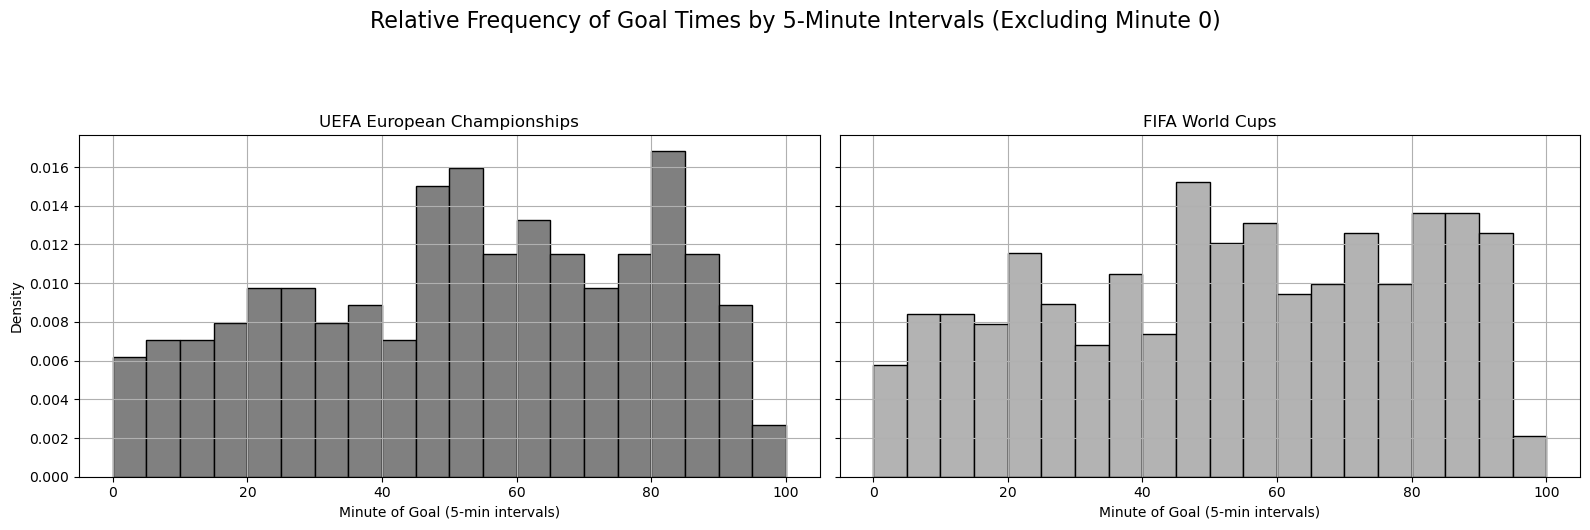
\includegraphics[width=1\textwidth]{images/gls_dist.png}
    \caption{Goals distribution Europe vs World Cup}
    \label{fig:gls_dist}
\end{figure}


To further understand the evolution of suspense over time, we classify the qualifications groups into stable and volatile depending on whether their average number of qualification changes lies below or above the median. This classification is then merged into the minute-by-minute dataset, allowing us to trace the trajectory of suspense separately for stable and volatile groups. In the European Championship under UEFA’s criteria (Figure~\ref{fig:susp_traj_eu_uefa}), the difference between the two trajectories appears minimal at the start and end of matches, while the largest gap emerges between the 30th and 50th minutes, with the gap averaging around 0.2 points overall. By contrast, under FIFA’s criteria (Figure~\ref{fig:susp_traj_eu_fifa}), the difference between stable and volatile groups starts at about 0.3 points and gradually narrows toward 0.2 points, with suspense steadily declining in both cases as time progresses.

\begin{figure}[H]
    \centering
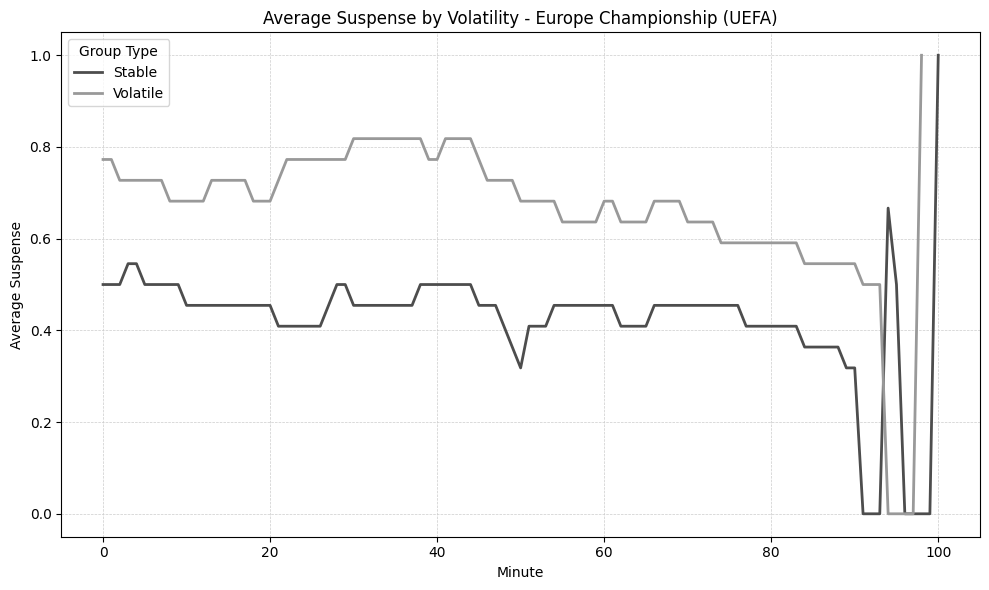
\includegraphics[width=1\textwidth]{images/susp_traj_eu_uefa.png}
    \caption{}
    \label{fig:susp_traj_eu_uefa}
\end{figure}

\begin{figure}[H]
    \centering
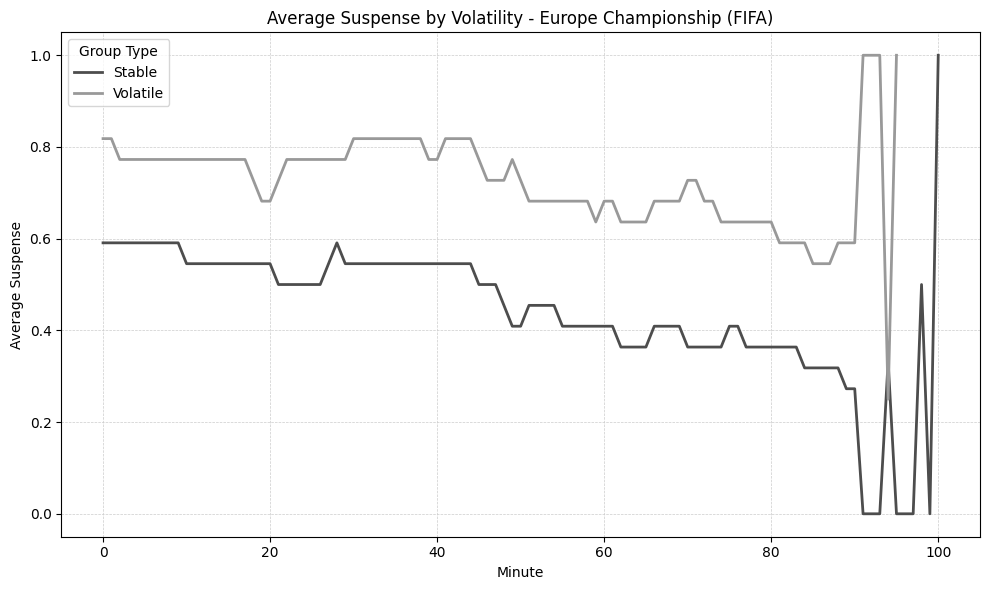
\includegraphics[width=1\textwidth]{images/susp_traj_eu_fifa.png}
    \caption{}
    \label{fig:susp_traj_eu_fifa}
\end{figure}


Turning to the World Cup, volatile groups exhibit higher levels of suspense under both criteria (Figures~\ref{fig:susp_traj_wc_uefa} and \ref{fig:susp_traj_wc_fifa}). Under FIFA’s rules, the gap is already substantial at the beginning of matches (around 0.4 points),  and remains large throughout, as both trajectories gradually decline over time. By contrast, under UEFA’s criteria the initial difference is more moderate (approximately 0.2 points), but it widens considerably as the match progresses. In particular, suspense in stable groups declines sharply toward the final minutes, while volatile groups retain relatively higher levels, leading to a pronounced late-match divergence.

\begin{figure}[H]
    \centering
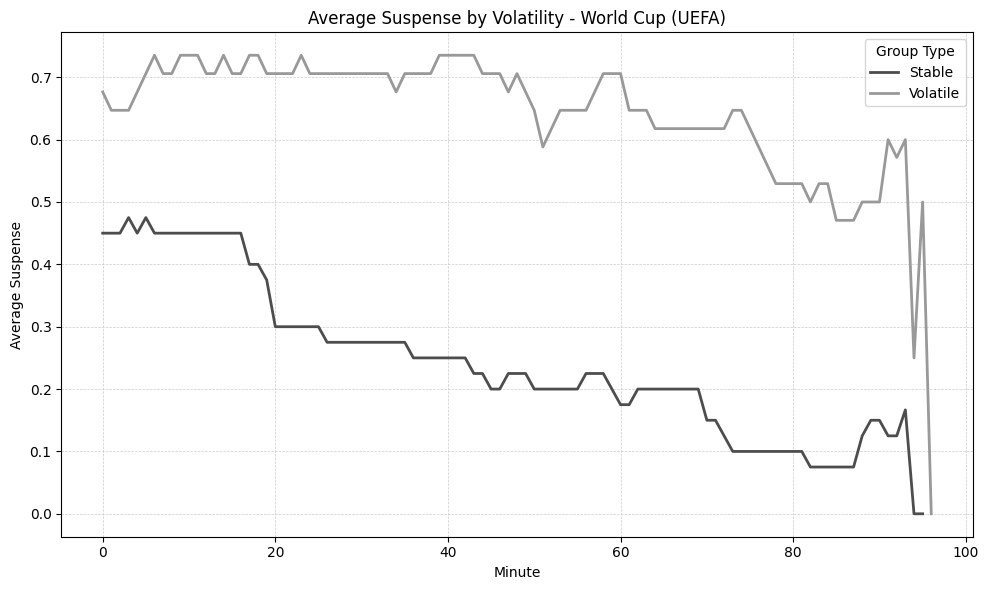
\includegraphics[width=1\textwidth]{images/susp_traj_wc_uefa.png}
    \caption{}
    \label{fig:susp_traj_wc_uefa}
\end{figure}

\begin{figure}[H]
    \centering
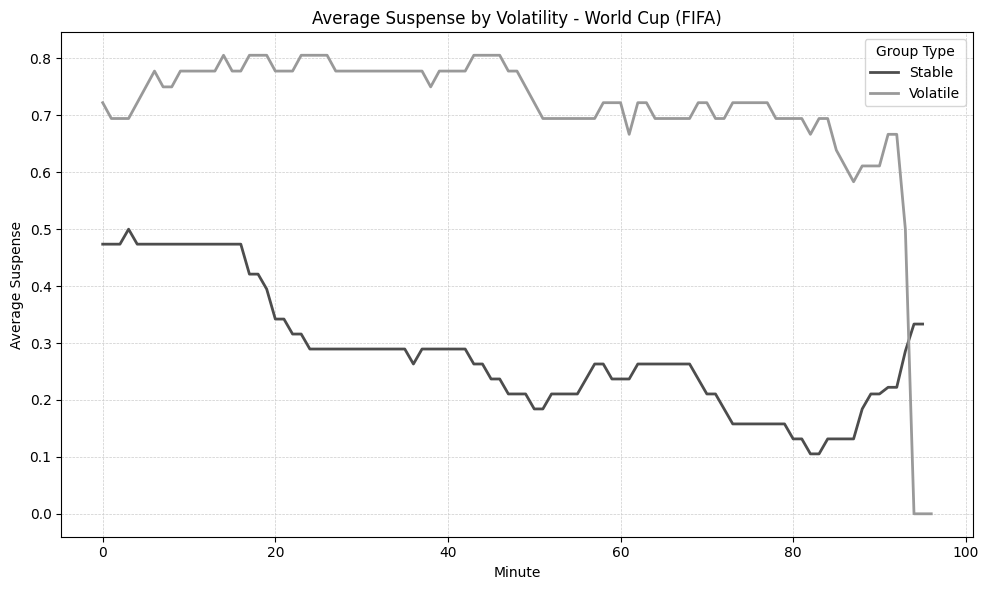
\includegraphics[width=1\textwidth]{images/susp_traj_wc_fifa.png}
    \caption{}
    \label{fig:susp_traj_wc_fifa}
\end{figure}

Taken together, these trajectories show that volatile groups systematically generate higher levels of suspense than stable ones, although the magnitude and timing of the divergence vary across competitions and tiebreaking systems. In the European Championship, the gap is moderate and most pronounced during the middle phase of matches, narrowing toward the end. By contrast, in the World Cup the difference is larger and more persistent, particularly under FIFA’s criteria, where volatile groups exhibit consistently higher suspense throughout the match.

\begin{figure}[H]
    \centering
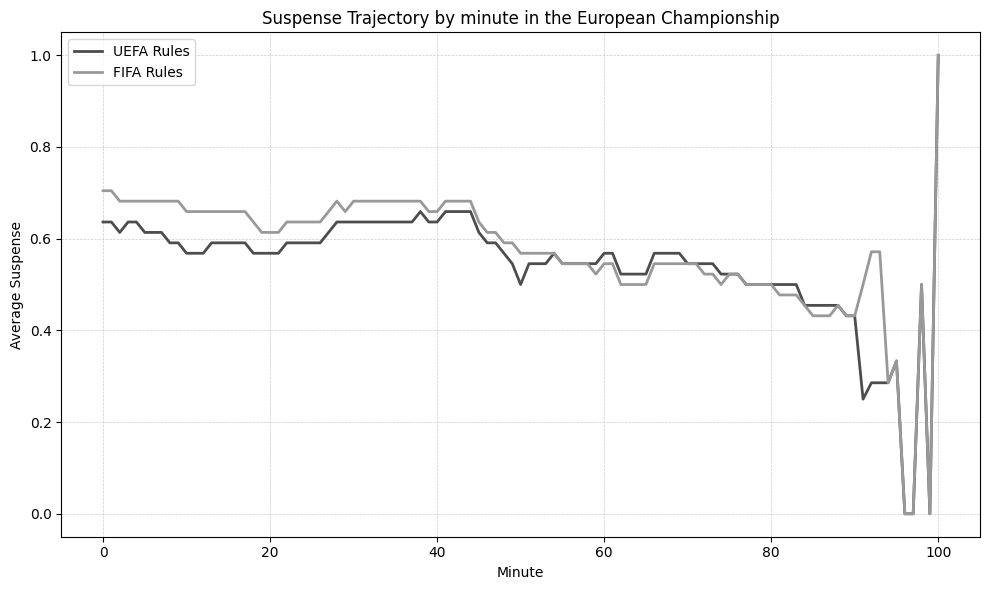
\includegraphics[width=1\textwidth]{images/susp_minute_eu.png}
    \caption{}
    \label{fig:susp_minute_eu}
\end{figure}

\begin{figure}[H]
    \centering
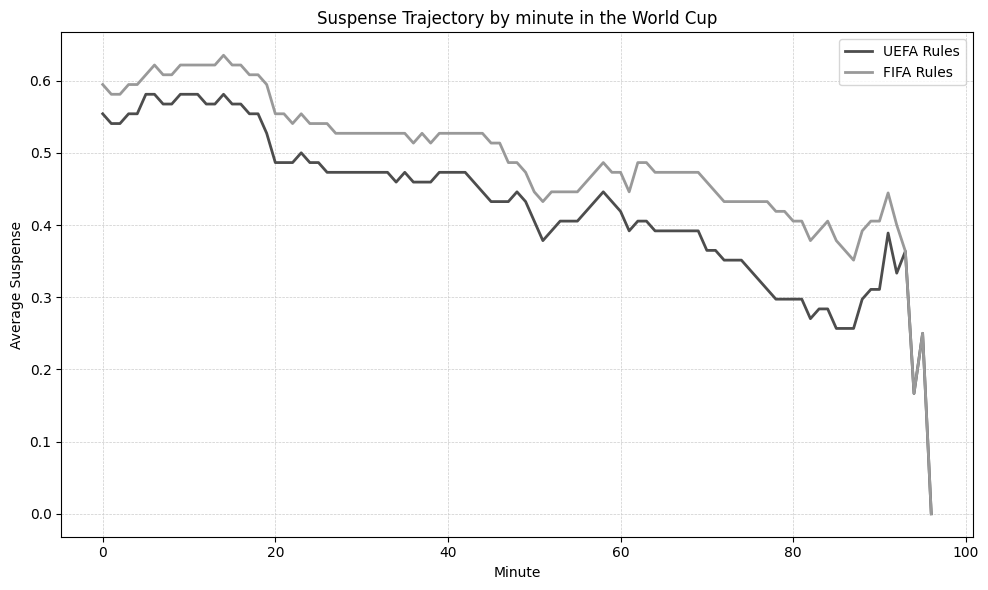
\includegraphics[width=1\textwidth]{images/susp_minute_wc.png}
    \caption{}
    \label{fig:susp_minute_wc}
\end{figure}

Figures~\ref{fig:susp_minute_eu} and \ref{fig:susp_minute_wc} display the average suspense per minute under FIFA and UEFA tie-breaking rules for the European Championship and the World Cup, respectively. In both cases, FIFA’s rules generate systematically higher suspense, with the gap being more evident in the European Championship, especially in the early stages of matches. At the same time, the overall level of suspense is higher in the World Cup than in the European Championship, regardless of the rule set applied. 

As highlighted in the statistical tests, FIFA’s tie-breaking rules systematically generate more suspense than UEFA’s. Combined with a more evenly goals distribution in the World Cup, this produces a setting where surprise is amplified - particularly in groups where the composition of qualifying teams changes frequently. In other words, both the institutional design of tie-breaking rules and the match dynamics of the World Cup contribute to making it the competition with the highest levels of perceived suspense.

\vspace{0.5em}
 
Our findings provide empirical support for \citet{csato2023avoid}, who, in analyzing the 2022/23 UEFA Nations League, argues from both a theoretical perspective and through simulated outcomes that prioritizing goal difference (FIFA criteria) over head-to-head results (UEFA criteria) raises the stakes of matches played toward the end of the competition. While FIFA’s system appears to promote competitiveness by incentivizing teams to score more goals, it is important to note that the number of matches where this rule meaningfully changes incentives is limited — though not negligible.

\subsection{Match level}

While at the group level the FIFA criteria (goal difference) generate more suspense by keeping a wider range of scenarios open, since a single goal affects the entire goal-difference tally rather than just the outcome of a single match, this results in group compositions changing more frequently and therefore higher suspense overall under FIFA rules.

\begin{figure}[H]
    \centering
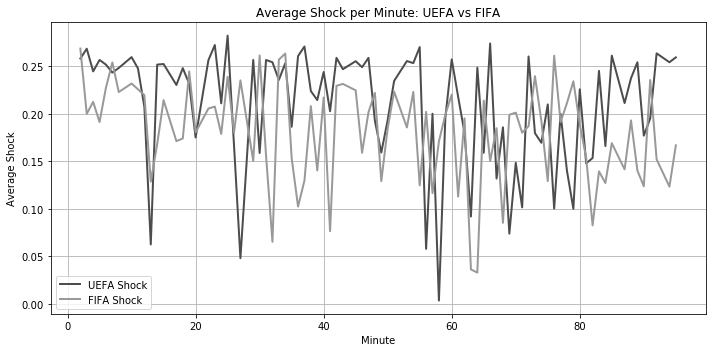
\includegraphics[width=1\textwidth]{images/shock.png}
    \caption{}
    \label{fig:shock}
\end{figure}


\begin{figure}[H]
    \centering
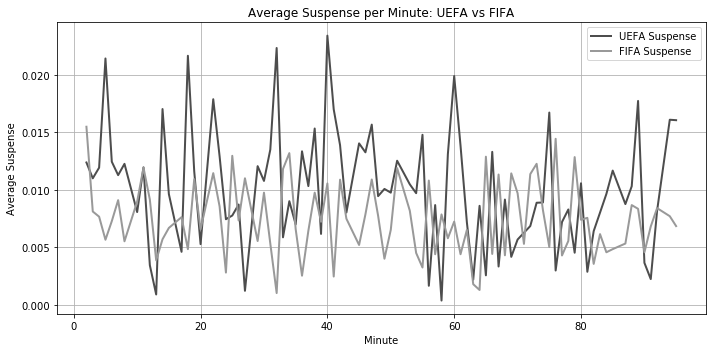
\includegraphics[width=1\textwidth]{images/suspense.png}
    \caption{}
    \label{fig:suspense}
\end{figure}


At the match level, however, as shown in Figures~\ref{fig:shock} and \ref{fig:suspense}, UEFA’s head-to-head criteria tend to produce greater suspense, shock, and surprise, along with larger fluctuations in these measures. This may be because prioritizing direct clashes amplifies the impact of goals in decisive matches: any goal that alters the head-to-head result can drastically shift a team’s qualification prospects.

Building on this point, it is worth noting that \citet{csato2023avoid} adopts a different approach to computing match probabilities. Instead of dynamically updating Elo-based win probabilities after each goal as we do, his framework derives goal expectations from Elo ratings using a Poisson model, where the expected number of goals for each team is estimated via a polynomial transformation of the Elo-derived win expectancy. To ensure comparability, we recalculated our suspense, surprise, and shock measures following this methodology. The resulting plots, reported in Figures~\ref{fig:shock_csato}, and \ref{fig:suspense_csato} in the Appendix, confirm the same patterns observed in our main analysis, reinforcing the conclusion that UEFA’s head-to-head criteria amplify match-level volatility relative to FIFA’s goal-difference rule.

Furthermore, we tried to combine the match-level suspense analysis with the group-level analysis by explicitly adjusting the underlying match probabilities when the qualification race was still on at group level. Specifically, we identify whether the third- or fourth-placed team in a group is already in contention or eliminated according to our binary indicator. If the team still in contention for the qualification is involved in the ongoing match, its win probability is tilted upward while the corresponding loss probability is reduced, while the draw probability remains approximately unchanged. This adjustment reflects the intuition that teams facing elimination may display greater motivation. We then recompute suspense, surprise, and shock based on these adjusted probabilities, ensuring that goal by goal dynamics evolve in line with group qualification dynamics. In this way, our match-level measures are directly linked to the group-level suspense of the qualification race under the two tie-breaking rules. Figures~\ref{fig:shock_agg} and \ref{fig:suspense_agg} confirms that UEFA tiebreak highlight all three measure (Surprise, Shock, Suspense) even when group dynamics are taken into account.

\begin{figure}[H]
    \centering
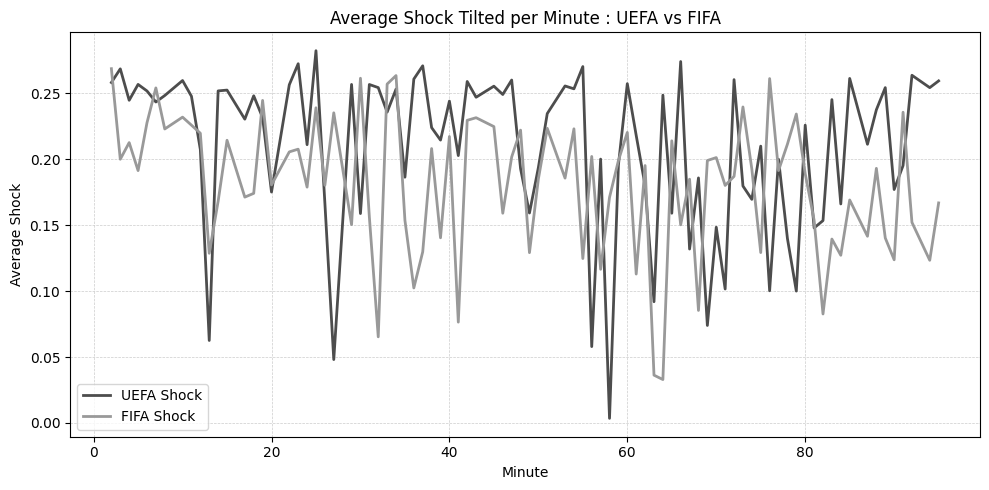
\includegraphics[width=1\textwidth]{images/shock_agg.png}
    \caption{}
    \label{fig:shock_agg}
\end{figure}


\begin{figure}[H]
    \centering
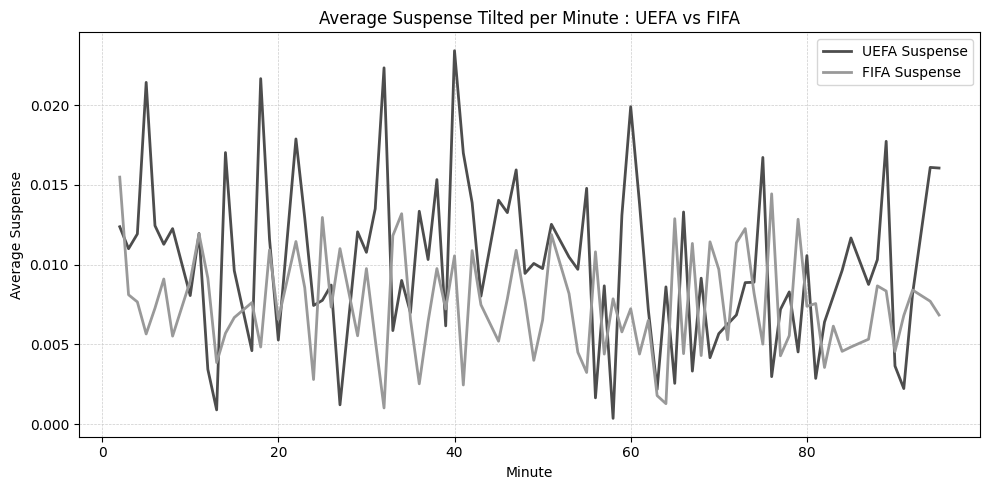
\includegraphics[width=1\textwidth]{images/suspense_agg.png}
    \caption{}
    \label{fig:suspense_agg}
\end{figure}

\section{Conclusion}
\label{sec: conclusion}


This paper was motivated by the desire to understand how alternative tie-breaking criteria shape the level of suspense in round-robin tournaments. Tie-breaking rules are not merely technical details: they influence the perceived attractiveness of games, with potential implications for revenues, stadium attendance, and viewership. By choosing one criterion over another, governing bodies implicitly decide whether to prioritize group-level or match-level dynamics.

We compared the two main approaches in international football: the FIFA rule, which prioritizes goal difference, and the UEFA rule, which prioritizes head-to-head results. Our analysis shows that these criteria generate systematically different patterns of suspense at the group level. Under the FIFA system, the average number of potential or actual changes in the qualifying teams’ composition following a goal is considerably higher. Likewise, the correlation between our mean value of compositional change of the qualifying teams  and the binary suspense measure is also stronger under FIFA rules. These descriptive findings are reinforced by statistical tests -- particularly for the European Championship -- where the probability of experiencing suspense is 12.5\% higher under FIFA’s goal-difference criterion.

To investigate how suspense unfolds throughout a match, we examined its minute-by-minute evolution. World Cup matches exhibit a more even distribution of goals and a sharper distinction between volatile and stable groups. Under FIFA rules, the distribution of suspense over the 90 minutes is more stable, and projected suspense per minute further supports the conclusion that FIFA tie-breakers generate more group-level suspense.

At the match level, however, UEFA’s head-to-head criterion amplifies measures of suspense, surprise, and shock. Because head-to-head results weigh heavily in determining qualification, goals in direct clashes can abruptly alter a group’s entire competitive landscape.

Overall, our results highlight that suspense can be defined and experienced not only within individual matches but also at the aggregate group level. Since fans typically understand the tie-breaking rules of the tournaments they follow, governing bodies should consider how different criteria affect the perceived attractiveness and interest of their competitions.

 


 
\bibliographystyle{apalike}
\bibliography{reference}
\appendix

\section{Appendix}
\subsection{Suspense Criteria: Full Logic}
\label{sec:suspense-criteria}

The following rules describe the exact criteria we use to assign a suspense value of 1 (suspenseful moment) in both FIFA and UEFA group stages. A suspenseful moment is defined as one where a single goal may change the composition of teams qualifying for the knockout stage. These rules are applied after each goal and at each match minute during the group stage.

\subsubsection*{Suspense Criteria: FIFA}
\label{sec:suspense-fifa-implemented}

FIFA ranking within the group follows the tie-break hierarchy:
\[
\text{Points} \;\; \rightarrow \;\; \text{Overall Goal Difference} \;\; \rightarrow \;\; \text{Overall Goals Scored} \;\; \rightarrow \;\; \text{Head-to-Head (if required)}.
\]
We evaluate suspense after each goal/minute observation using the pipeline below.

\paragraph{Step 0: Identify the cut-off pair (leading vs lagging).}
Let \texttt{third\_qualify} indicate whether the relevant cut-off is:
\begin{itemize}
    \item \texttt{third\_qualify = 0}: \textbf{2nd} (leading, last qualified) vs \textbf{3rd} (lagging, first not qualified),
    \item \texttt{third\_qualify = 1}: \textbf{3rd} (leading) vs \textbf{4th} (lagging).
\end{itemize}
We denote the lagging and leading teams’ current \emph{overall} differences by:
\[
\texttt{pts\_diff}_0,\;\texttt{gls\_diff}_0,\;\texttt{gs\_diff}_0,
\]
where \texttt{gs\_diff} is computed as goals scored by lagging minus goals scored by leading.

\paragraph{Step 1: Infer current match points from match goal difference.}
At every minute, each team has a match-specific goal difference (\texttt{last\_game\_goals\_diff}). 
We infer match points robustly from this match GD:
\[
\texttt{match\_pts} =
\begin{cases}
\texttt{win\_pts} & \text{if match GD} > 0,\\
1 & \text{if match GD} = 0,\\
0 & \text{if match GD} < 0,
\end{cases}
\]
with \texttt{win\_pts} $=2$ if \texttt{year $\le$ 1992} and \texttt{win\_pts} $=3$ otherwise.

\paragraph{Step 2: Evaluate the two one-goal shocks (\texttt{calculate\_suspense}).}
We compute whether \emph{either} of the following shocks makes lagging rank $\ge$ leading under FIFA ordering:
\begin{enumerate}
    \item \textbf{Lagging scores (+1)}.
    \item \textbf{Leading concedes (+1)}.
\end{enumerate}

\noindent The shocks update \emph{both} (i) match states and (ii) overall differences:
\begin{itemize}
    \item If \texttt{h2h = 0} (teams are in different matches), the shock affects only the relevant team’s match GD by $\pm 1$ and hence may change match points. Overall GD changes by $+1$ in favor of lagging for either shock. Goals scored changes by $+1$ \emph{only} if lagging scores.
    \item If \texttt{h2h = 1} (teams are facing each other in the current match), a single goal simultaneously improves lagging’s match GD by $+1$ and worsens leading’s match GD by $-1$. Hence overall GD changes by $+2$ in favor of lagging. Goals scored of lagging increases by $+1$.
\end{itemize}

\noindent After updating points (through inferred match points), overall GD, and overall goals scored, suspense is set to 1 if lagging becomes \emph{not behind} leading under:
\[
\text{Points} \rightarrow \text{Overall GD} \rightarrow \text{Overall GS}.
\]
If the shock produces a full tie on all three dimensions, we still classify the moment as suspenseful (\texttt{suspense=1}), since the next tie-break (e.g., head-to-head or lots) may decide qualification.

\paragraph{Step 3: Flag head-to-head tie-break cases (\texttt{update\_suspense}).}
We create the indicator \texttt{h2h\_suspense} to identify the subset of observations where the qualification cut-off would be decided by the \emph{head-to-head} tie-break between the lagging and leading teams.
Operationally, we flag \texttt{h2h\_suspense=1} when a full tie on the \emph{FIFA pre-H2H criteria} (points, overall goal difference, and overall goals scored) can be reached with a single-goal shock from \emph{both} perspectives:
\begin{itemize}
    \item full tie after \textbf{lagging scores (+1)}, and
    \item full tie after \textbf{leading concedes (+1)}.
\end{itemize}
Only for these cases we set \texttt{suspense=1} and \texttt{h2h\_suspense=1}. 
This ``both perspectives'' requirement excludes situations where only one shock produces a full tie, while the other shock would already give one team a strict advantage on goals scored.

\paragraph{Step 4: Evaluate the relevant head-to-head match (\texttt{evaluate\_lagging\_losses\_and\_update\_suspense}).}
For observations with \texttt{h2h\_suspense=1}, we evaluate the head-to-head status between the lagging and leading teams to determine whether the tie-break can actually favor the lagging team.
There are two distinct cases:
\begin{itemize}
    \item \textbf{\texttt{h2h = 1} (current match):} lagging and leading are facing each other in the ongoing match. In this case, the head-to-head outcome is determined by the \emph{current score} at minute $t$ (i.e., the current match goal difference for the lagging team).
    \item \textbf{\texttt{h2h = 0} (previous match):} lagging and leading are not playing each other in the current match minute; their head-to-head match is in the one of the \emph{previous} fixture in the same group stage. In this case the head-to-head outcome is fixed and can be retrieved from \texttt{goals\_df} using the match’s final score. If the lagging team loses the head-to-head match, we set \texttt{suspense} back to 0 for that observation.
\end{itemize}
\paragraph{Step 5: Draw-lots adjustments (\texttt{update\_suspense\_draw\_lots}).}
Finally, we manually set \texttt{suspense=1} in a small set of edge cases where the FIFA rules imply qualification may be decided by lots.

\paragraph{Diagnostic audit: outside-team threat when \texttt{suspense=0} (\texttt{audit\_suspense0\_where\_4th\_threatens\_2nd\_fifa}).}
Because the main suspense logic evaluates only the cut-off pair (leading vs lagging), we also run a diagnostic check for cases with \texttt{suspense=0} and \texttt{third\_qualify=0} where the \textbf{4th} team can reach or overtake the \textbf{2nd} team with one goal shock under FIFA ordering. This audit:
\begin{itemize}
    \item does \emph{not} use \texttt{pts\_diff} or \texttt{gls\_diff} (they refer to the main pair),
    \item compares \textbf{4th vs 2nd} using their own points/GD/GS and match states,
    \item handles the special case where 2nd and 4th are playing each other (shock affects both match states and overall GD by $+2$).
\end{itemize}
The audit returns the subset of rows where such an outside threat exists, to allow the manual correction of the suspense dummy.

\subsubsection*{Suspense Criteria: UEFA}
\label{sec:suspense-uefa-implemented} For competitions governed by UEFA rules, team ranking within a group follows a different tie-breaking hierarchy than FIFA. Teams are ranked according to:
\begin{enumerate}
    \item total points,
    \item head-to-head result between the tied teams,
    \item overall goal difference,
    \item overall goals scored.
\end{enumerate}
Unlike the FIFA procedure, head-to-head is applied \emph{before} overall goal difference and goals scored.

\paragraph{Step 1: Identify the relevant ranking pair.}
At each observation (defined by a goal minute within a group-stage match), we identify the pair of teams defining the qualification cut-off. When only the top two teams qualify (\texttt{third\_qualify = 0}), the relevant comparison is between the teams ranked second and third. When the third-placed team may also qualify (\texttt{third\_qualify = 1}), the relevant comparison is between the teams ranked third and fourth. The lower-ranked team in this pair is denoted as the \emph{lagging} team and the higher-ranked team as the \emph{leading} team.

\paragraph{Step 2: Evaluate one-goal shocks.}
For each observation we evaluate whether a single-goal shock could allow the lagging team to reach or overtake the leading team in the ranking. Two possible shocks are considered:
\begin{itemize}
    \item \textbf{Lagging scores one goal (+1).}
    \item \textbf{Leading concedes one goal (+1).}
\end{itemize}

If the lagging and leading teams are playing each other in the current match (\texttt{h2h = 1}), the shock affects both teams simultaneously (lagging goal difference increases by one and leading goal difference decreases by one). If the teams are playing in different matches (\texttt{h2h = 0}), the shock affects only the relevant team's match state.

Match points are inferred from the match goal difference at the current minute using the appropriate points system (two points for a win before 1993 and three points thereafter).

\paragraph{Step 3: Apply UEFA tie-breaking rules.}
After applying the hypothetical shock, we compare the lagging and leading teams according to the UEFA ranking hierarchy.

First, we evaluate the difference in total points. If the lagging team would have strictly more points, the lagging team overtakes the leading team and suspense exists.

If the teams would be tied on points, the next criterion is the head-to-head result between the two teams. When the two teams are not currently facing each other (\texttt{h2h = 0}), we use the indicator \texttt{lagging\_won}, which takes value:
\begin{itemize}
    \item $1$ if the lagging team won the head-to-head match,
    \item $-1$ if the lagging team lost,
    \item $0$ if the head-to-head match was drawn.
\end{itemize}
If the lagging team won the head-to-head match, it ranks ahead and suspense is set to 1; if it lost, suspense is set to 0.

If the head-to-head match ended in a draw (\texttt{lagging\_won = 0}), the ranking falls back to overall goal difference and then overall goals scored. 
When the teams are currently facing each other (\texttt{h2h = 1}), we do not use \texttt{lagging\_won}; instead, we infer the \emph{current} head-to-head outcome from the live match goal difference (win/draw/loss for the lagging team). If the current head-to-head outcome is a win or a loss, it is decisive at the head-to-head step; if it is a draw, we proceed to overall goal difference and overall goals scored.

\paragraph{Step 4: Determine suspense.}
If under either of the two one-goal shocks the lagging team becomes at least as well ranked as the leading team according to the UEFA hierarchy, the observation is classified as a suspenseful state and we set \texttt{suspense = 1}. Otherwise, suspense remains equal to zero.

\paragraph{Step 5: Identify outside-team threats.}
Finally, we perform an additional audit to detect cases where suspense is equal to zero for the main pair but an \emph{outside team} could still affect the qualification boundary. Specifically, we check whether the fourth-placed team could reach or overtake the second-placed team with a single-goal shock, again applying the UEFA ranking hierarchy (points, head-to-head, goal difference, goals scored). Observations satisfying this condition are edit separately to assess whether the suspense variable should be adjusted.

\subsection{Match Dynamics and Bookings Adjustments}
\label{sec: bookings}

To incorporate match dynamics and disciplinary events, we adapt the framework of \citet{titman2015joint}, who jointly model goals and bookings in football matches. Specifically, we implement a set of rules that adjust the baseline Elo-derived win probabilities according to in-game events:

\begin{itemize}
    \item \textbf{Yellow cards}: Each yellow card reduces the affected team's win probability by \(-0.01\), reflecting reduced squad stability and heightened risk of further sanctions.
    \item \textbf{Red cards}: Straight red cards impose a stronger penalty of \(-0.04\). Second yellow (indirect red) cards impose a penalty of \(-0.03\), with an additional adjustment of \(0.015 \times \log(\text{number of prior yellow cards})\), accounting for accumulated fouls.
    \item \textbf{Substitutions}: Each substitution provides a small positive adjustment of \(+0.01\), representing tactical flexibility and fresh player input.
    \item \textbf{Escalation effects}: When one team accumulates at least one card, the opponent also receives a minor penalty of \(+0.005\), accounting for retaliation risk and increased match tension.
    \item \textbf{Scoreline adjustments}: Leading teams receive a reduction of \(-0.005\) per goal ahead (safer play), while tied matches add a penalty of \(+0.003\) for both teams, reflecting greater competitive tension.
\end{itemize}


\subsection{Additional Figures}
\begin{figure}[H]
    \centering
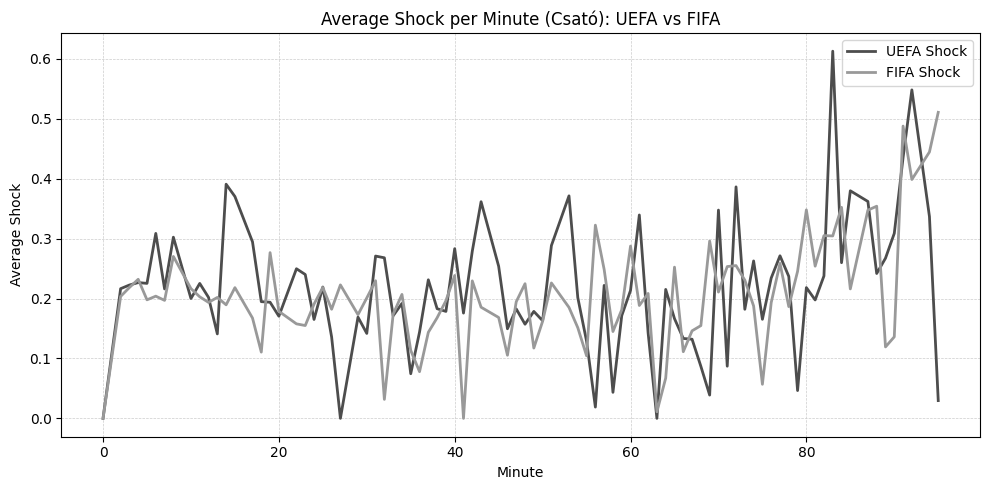
\includegraphics[width=1\textwidth]{images/shock_csato.png}
    \caption{}
    \label{fig:shock_csato}
\end{figure}


\begin{figure}[H]
    \centering
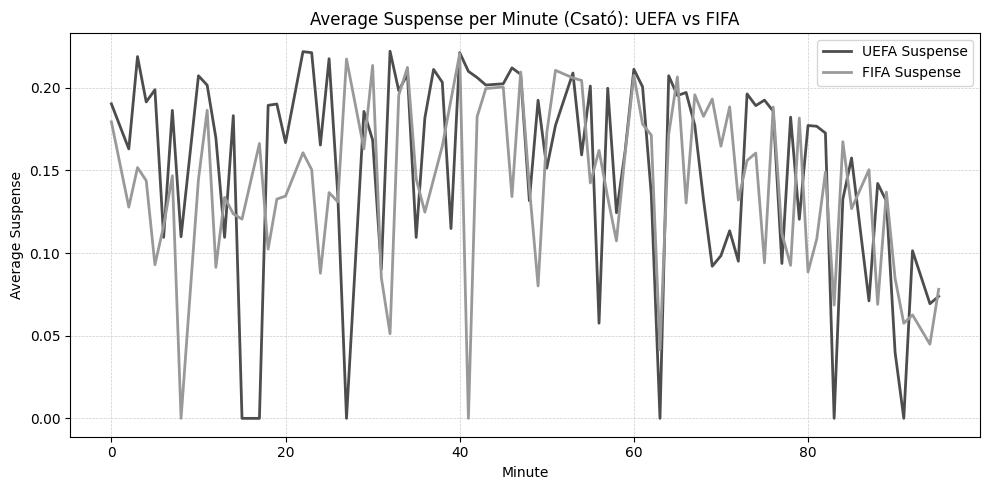
\includegraphics[width=1\textwidth]{images/suspense_csato.png}
    \caption{}
    \label{fig:suspense_csato}
\end{figure}


\end{document}
